%!TEX root = manual.tex
%===============================================================================
\chapter{Tasking housekeeping program}\label{ch:Assignment4}

The aim of this assignment is to extend the simple housekeeping program of the previous assignment by adding a communications subsystem. The extended system includes two concurrent tasks communicating through a protected shared object.

\section{Software architecture}

The software architecture of the tasking housekeeping program is depicted in figure~\ref{fig:tasking}. The software components are:

\begin{figure}[h]
            \centering{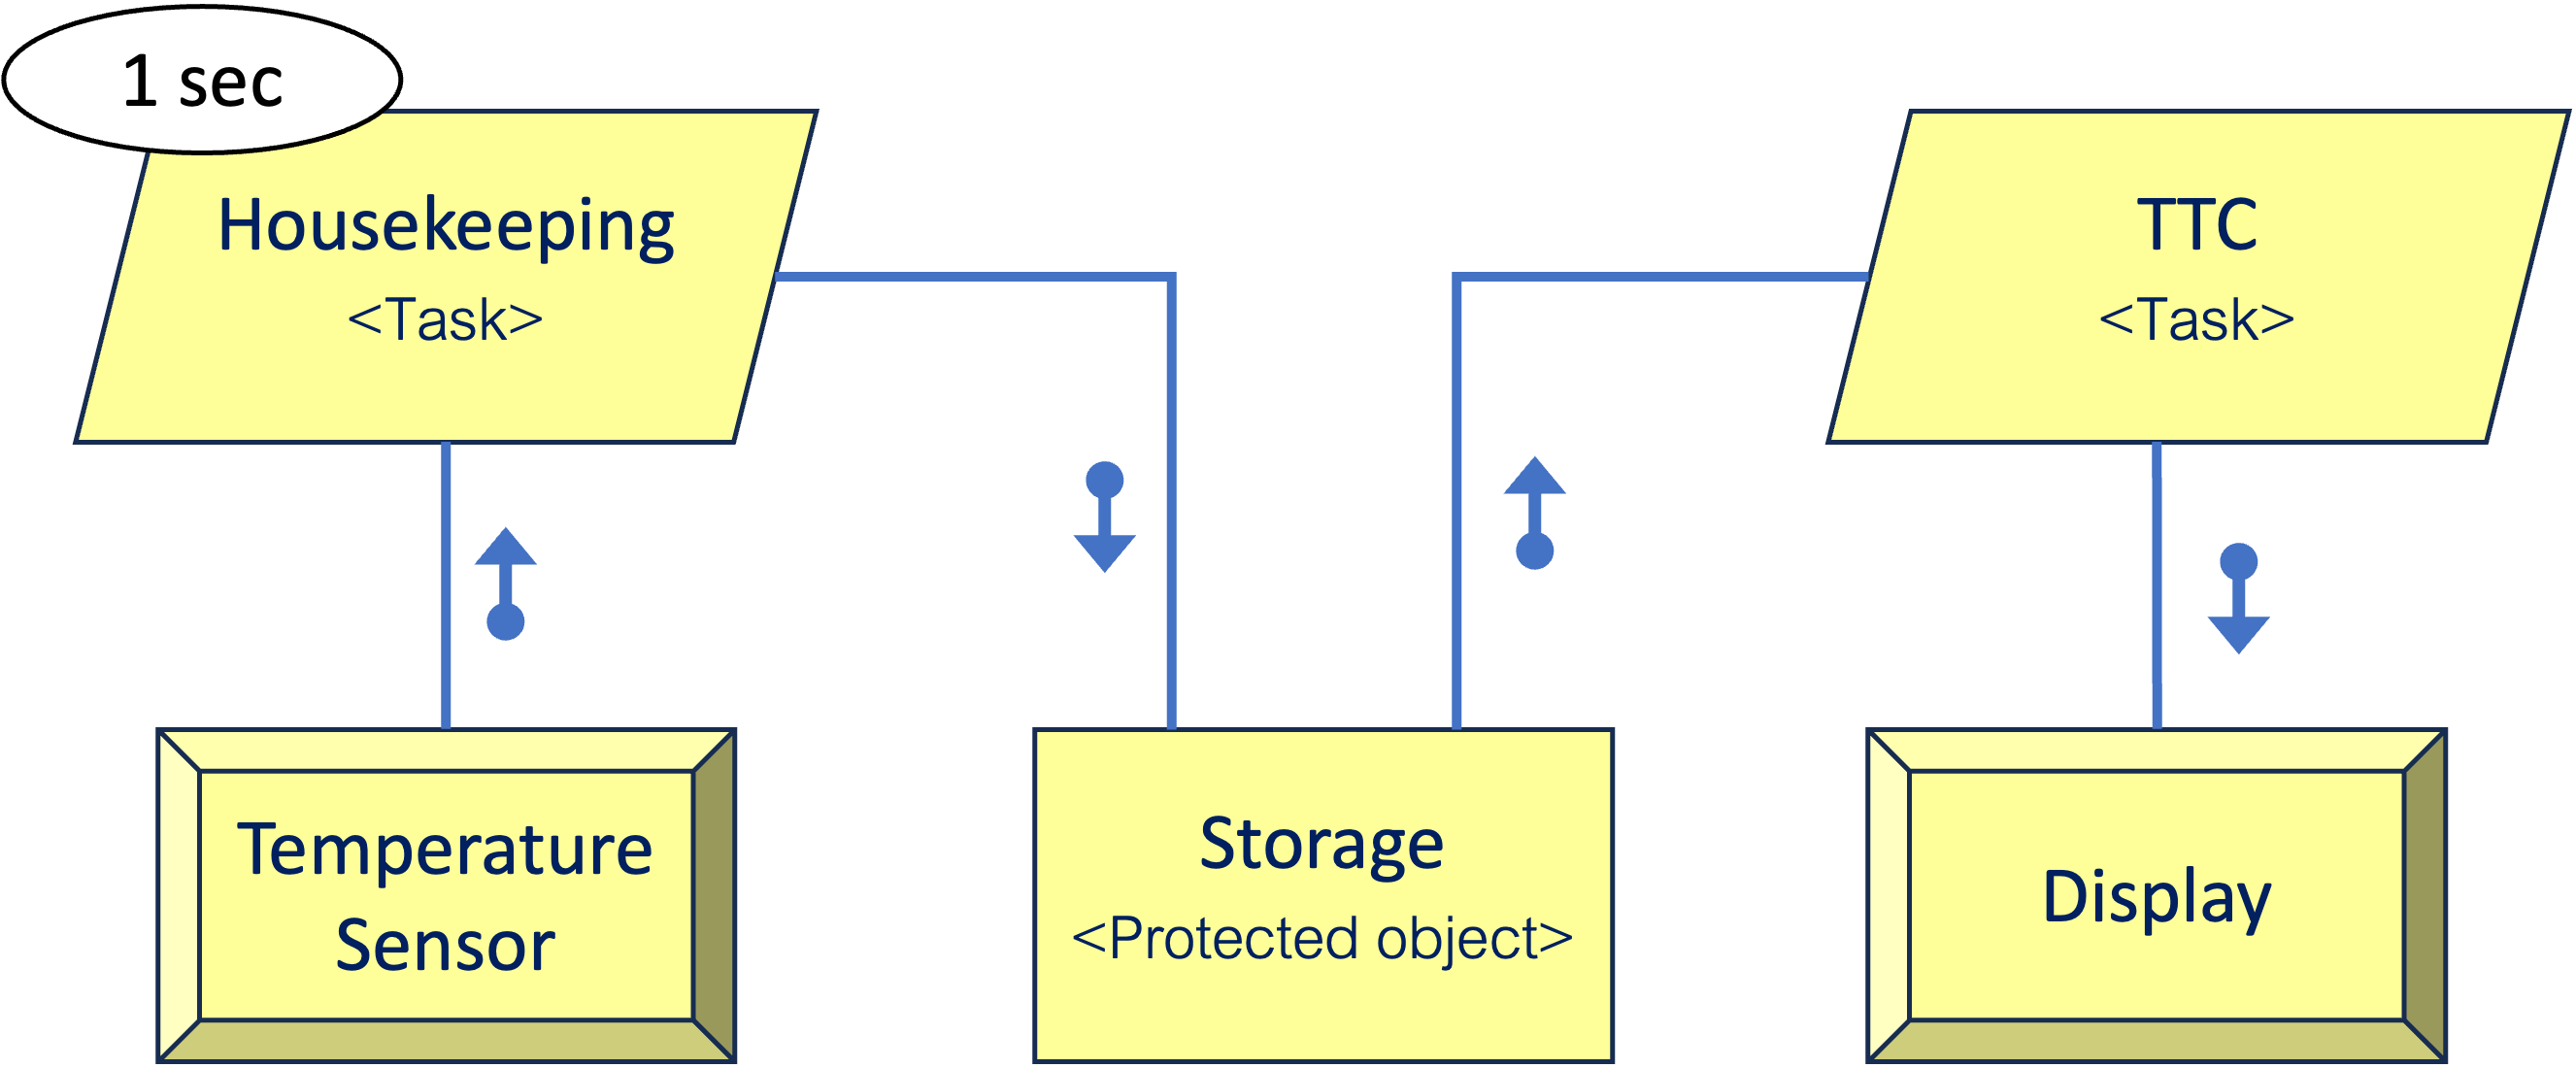
\includegraphics[width=.9\textwidth,keepaspectratio]{tasking.png}}
            \caption{Software architecture of tasking housekeeping system.}
            \label{fig:tasking}
\end{figure}

The differences with the previous architecture are:
\begin{itemize}
\item There is a new component, {\tt TTC}, that handles the display.
\item Both the {\tt Housekeeping} and {\tt TTC} components include concurrent tasks.
\item The {\tt Housekeeping} and {\tt TTC} tasks communicate through a new component, {\tt Storage}. This component is a data object storing one temperature value, which is written by {\tt Housekeeping} and read by {\tt TTC}.
\end{itemize}

\subsection{Download the code and study the implementation}

The implementation code, as initially provided to the students, can be downloaded from \url{https://github.com/STR-UPM/OBDH\_LABS}. Click on {\tt Clone} or {\tt download}, download a zip archive, unzip and move to your work directory. The code for this assignment is in the LAB4 folder.

As in the previous assignment, the {\tt Housekeeping} package is the root element of the housekeeping subsystem. Its specification and body is similar to the previous version, except that it now contains a concurrent task, {\tt Housekeeping\_Task}, and the values read from the sensor are sent to {\tt Storage} instead of {\tt Display}. This package has been moved to the {\tt TTC} subsystem, but otherwise remains similar.

The {\tt TTC} package is the root of the telecommunications system, which in this version is greatly simplified with respect to a real application. It contains a concurrent task, {\tt HK\_Task}, which takes measured sensor values from {\tt Storage} and puts them on the display.

The {\tt Storage} package implements the communication between the {\tt Housekeeping} and {\tt TTC} subsystems.  Since this object is shared by two concurrent tasks, it is implemented as a protected object, so that its operations are executed in mutual exclusion. There is also conditional synchronization: the {\tt TTC} task must wait until there is a fresh value in the store. However, {\tt Housekeeping} should not wait if the previous value put into {\tt Storage} has not been consumed, in order not to delay the housekeeping function. In this case, the stored value is overwritten. Notice that this differs from the classical specification of a bounded buffer.

The {\tt OBSW} main procedure initialises the board LEDs and the {\tt Housekeeping} and {\tt TTC} subsystems toggle blue and orange LEDs.  The activity of both subsystems is carried out by their respective tasks, which start executing concurrently with the main task. The initialization procedures return to the main procedure, which enters an endless loop doing nothing and running in parallel with the other tasks. In order not to disturb the execution of the subsystems tasks, the main loop runs at the lower possible priority, which is specified in the {\tt obsw.ads file.}

\section{Compile and run with the debugger.}

Open GPS and do the following:
\begin{enumerate}
\item Select {\tt Open project} on the welcome window. Navigate to the LAB4 directory and open the {\tt tasking\_housekeeping.gpr} project file.

\item Build the executable and load it into the board by clicking on the \hbox{\includegraphics[width=1.5em]{debug.png}} symbol in the tool bar (or select {\tt Build} $\rightarrow$ {\tt Bareboard} $\rightarrow$ {\tt Debug} on board on the top menu).

The program will be compiled, and the executable will be loaded into the board memory by the debugger. After that, the debugger is started, and the debugger console (lowest window in GPS) shows the following lines:
\begin{verbatim}
...
(gdb) monitor reset halt
(gdb)
\end{verbatim}

\item Type {\tt continue} or just {\tt c} on the debugger console (or select {\tt Debug} $\rightarrow$ {\tt Continue} on the top menu).
\begin{verbatim}
(gdb) c
Continuing.
[program running]
\end{verbatim}

\item The program will start running (check the LED blinking), and the raw temperature readings are shown on the {\tt Messages} tab of the debugger console as in the previous project.
\end{enumerate}

\section{Make changes to the program}

It is advised that you make changes
to the provided program in order to make sure
that you understand the project implementation,
and the mapping from the architecture to source code.

\textcolor{mRedBrown}{\textit{The proposed change is to}}: Include the conversion to Celsius in the \texttt{TTC.Send} procedure.
The temperature transfer function is implemented by \texttt{HK\_data-converter}
which can be found in utilities.
